\section{Methods} \label{Methods}
This Section covers our adaptive narrative PCG model in Subsection \ref{Adaptive PCG Model}. Then, Subsection \ref{Renpy} covers the visual novel engine Renpy, used for our game prototype. Finally, Subsection \ref{Karma History Prototype} presents the prototype and some screenshots from a playthrough.

\subsection{Adaptive PCG Model} \label{Adaptive PCG Model}
The game keeps track of event history and user personality in a global history object. A short pre-game segment is used to determine a player's starting personality and placement tags. Once a player completes the initial segment, the game will transition to different events based on pre/postconditions. Events form a directed graph where events that have post-conditions that are a subset of another event's pre-conditions from a link to that event. Events will randomly transition to any event in which their post-condition tags are a subset of another event's pre-condition tags. Player choices in an event sometimes add tags to that event's post-conditions before the possible edges are calculated.

\begin{figure*}[ht]
    \centering
    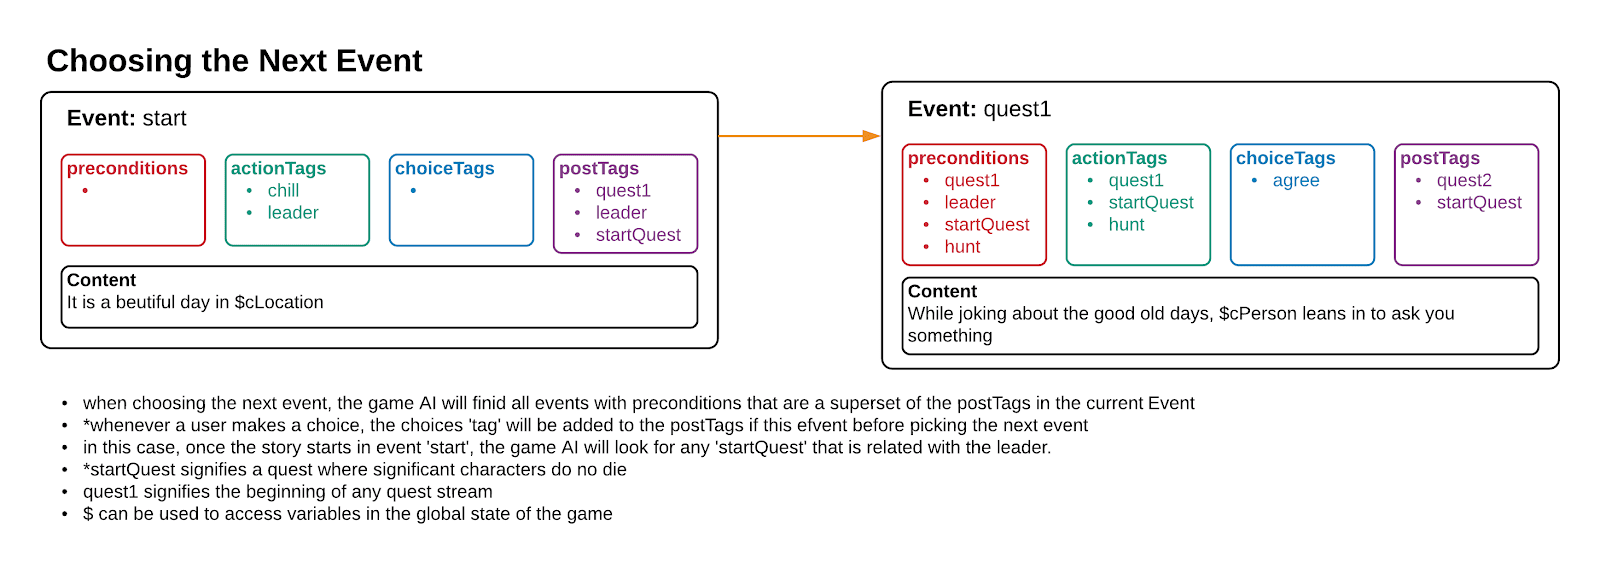
\includegraphics[width=\textwidth]{images/eventChoice.png}
    \caption{How an event is chosen}
    \label{fig:eventChoose}
\end{figure*}

Actions and NPCs (Non-Player Characters) appearing in events are determined with a tag system. The tag system can reference the global history structure to recall a previous choice or check if a condition has been met. Events contain separate tags to decide NPC actions and player choices. Not every event has to have either an NPC action or player choice; some include text to reflect on the outcome of the previous event/choice combination. NPC actions and player choices are chosen the same way as events, action and choice tags in an event must be a subset of the tags in the Action and Choice objects. An Event will randomly pick a suitable action and choice if possible. Actions also have a set of tags used to pick suitable NPCs for that action. 

\begin{figure*}[ht]
    \centering
    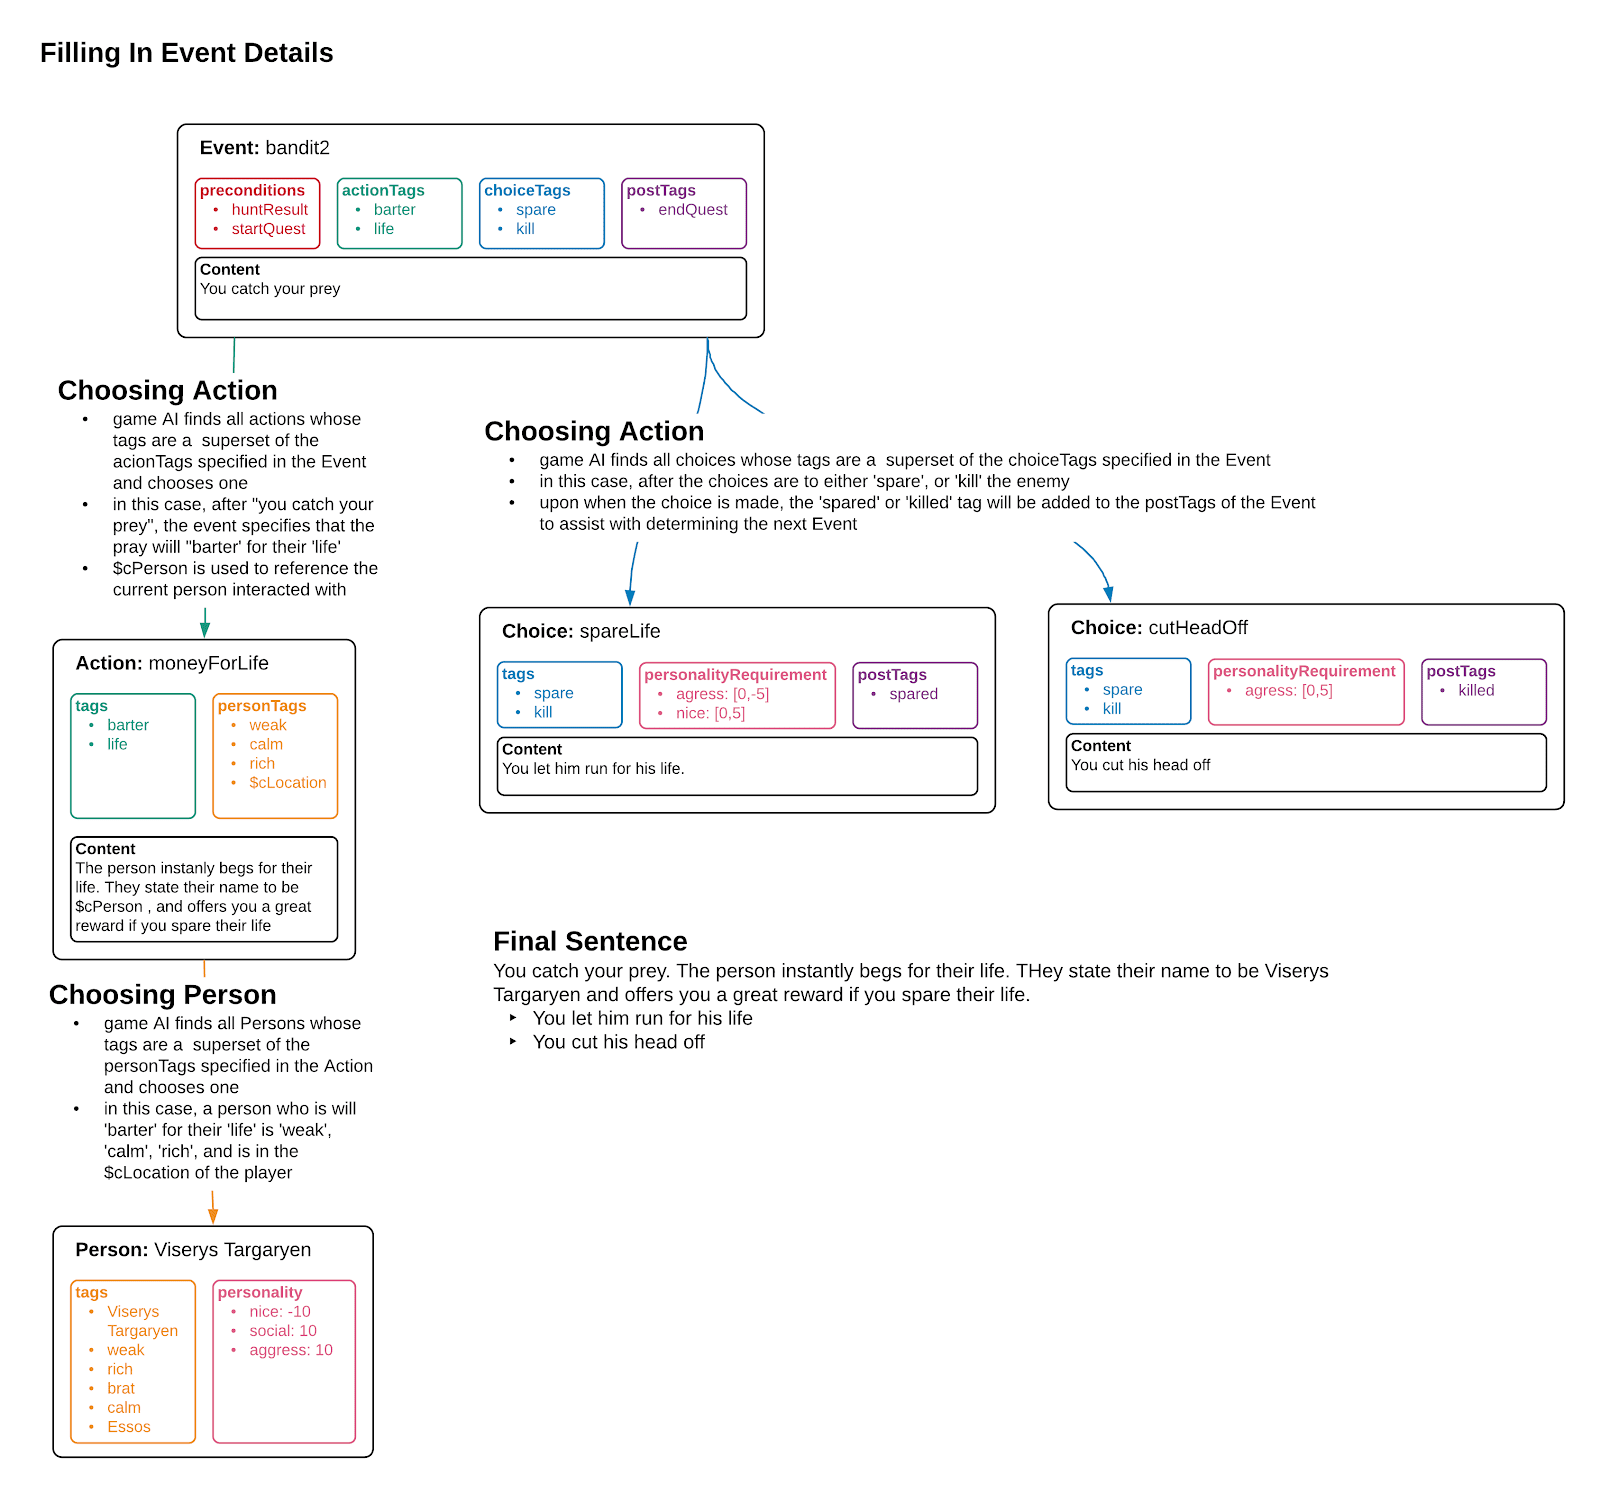
\includegraphics[width=\textwidth]{images/eventFill.png}
    \caption{How an event is broken down}
    \label{fig:eventFill}
\end{figure*}

NPC actions contain text describing what an NPC is doing. The presence of a set of person tags is to guarantee that a suitable NPC is picked for the action. For example, we never want a greedy character giving the player money for no reason. Every NPC character made for the game has unique personality values like the player, along with a set of tags that should specify their personality and background. The person chosen for an action is chosen the same way an action is, an NPC's tags must be a superset of the person tags in the Action object. An action is only suitable if at least one suitable NPC is found. The latest character chosen by an NPC action is saved to the global history, so it is not always necessary to generate a new action/character tag at every event. This allows developers to guarantee specific event lines when desired, allowing for scenes spanning several conversation points.

Choice objects contain text specifying what the player is doing in that choice, tags to be picked by an event, a personality requirement in order to be used by a player, a value to modify the player's personality if chosen, and any amount of post-tags to added to the event's post tags if chosen. The optional post tags are used to mark significant decisions, such as the death of a major character. These post tags can also be used to alter the global game state by adding/removing tags from NPC characters. This is essential to ensure that events transition appropriately based on choices.

There are many possible combinations of actions and people when the two objects are written as intended. This makes the tag system paramount to the results of narrative generation in Karma History. We already make use of two special tags in the game. The \$ tag retrieves a specified variable from the global history; this is used to fill in names, actions, and choices from previous events. The \# is used for a pre-condition global history check by events. It was unfeasible to grow the tags passed by an event's continuously, so we use \# tags to block progression to points of the story that do not make sense given the current global state. \#tags are removed from an event's pre-condition once the global condition they specify is met.

\subsection{Renpy} \label{Renpy}
We used Renpy \cite{renpy} to implement a prototype for this model. Renpy is a visual novel engine that displays an image in the background and text as shown in Figure \ref{fig:customLannister}. The text field can present choices, text entry fields, or just strings. It is built on top of Python \cite{python} allowing for embedded python scripts within the Renpy scripting language.

Renpy was chosen for this project because it was lightweight, simple, and provides the basic features for a narrative game. Its ability to include embedded Python was the biggest factor in creating a quick prototype. Python is a common language we both already knew with quick setup time. Learning a new system such as Unity \cite{unity} was desired, but would take too long to learn.

\subsection{Karma History Prototype} \label{Karma History Prototype}
To prototype our Adaptive PCG model with Renpy, we created a game called Karma History, based on Game of Thrones \cite{got}. This prototype is a proof of concept for our model through the surveys in section \ref{Results}. Figures \ref{fig:menu} to \ref{fig:customLannister} show Karma History at different points in the game. 

\begin{figure}[ht]
    \centering
    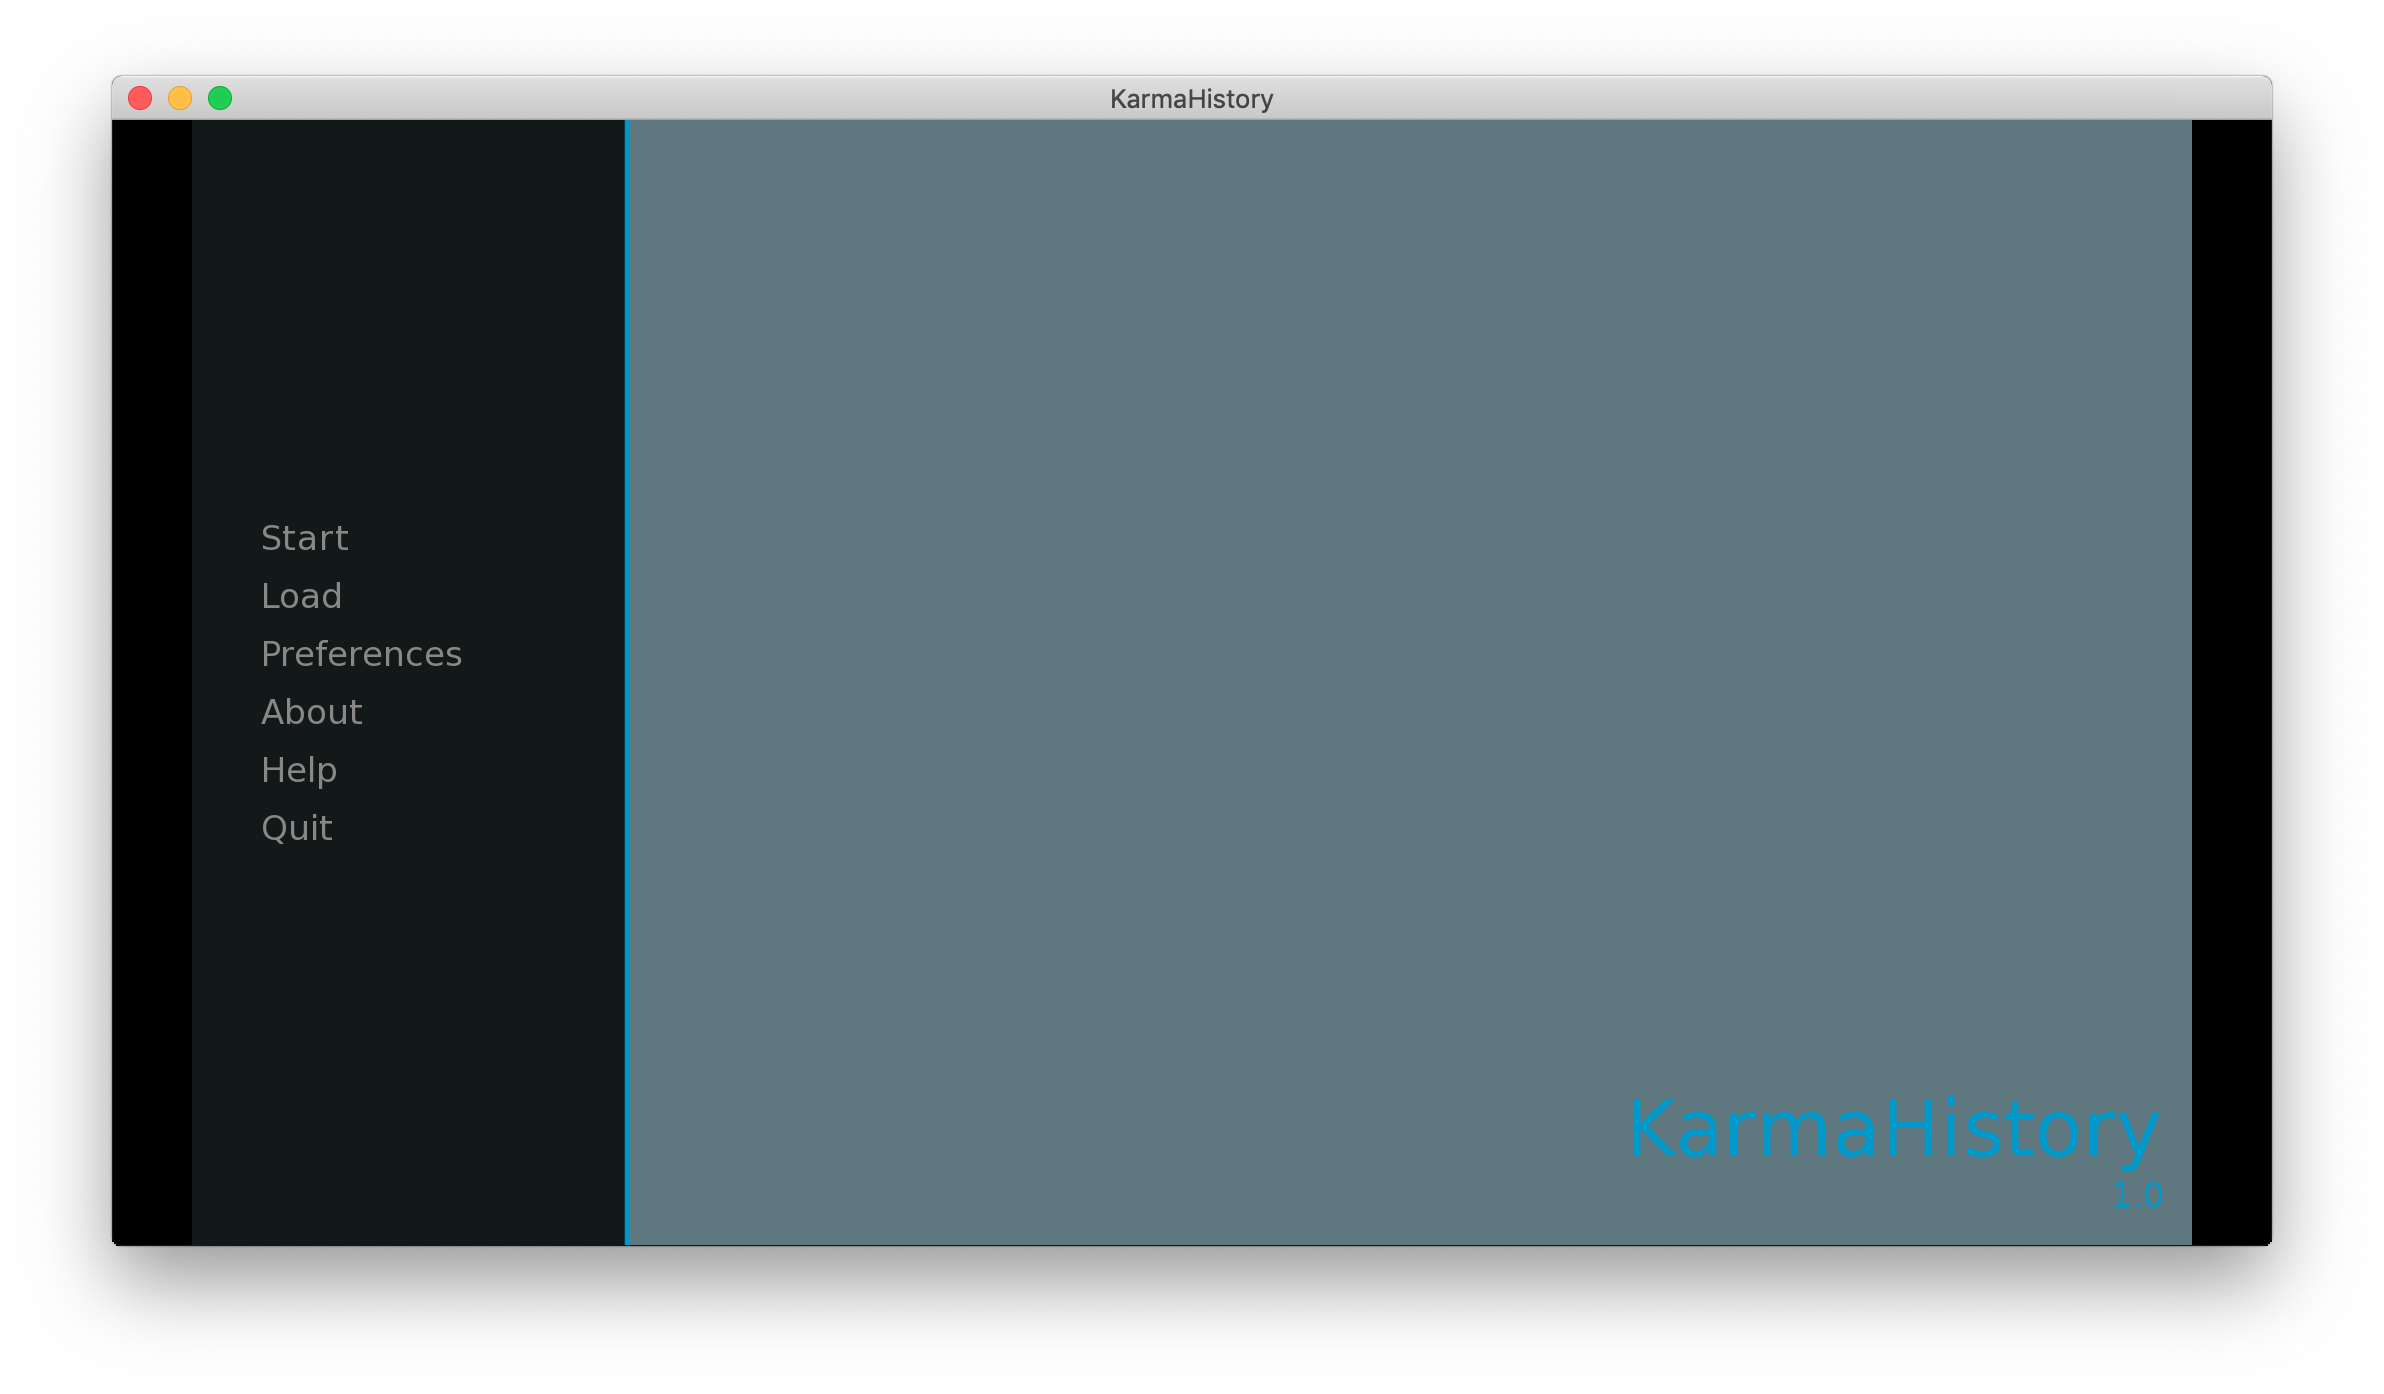
\includegraphics[width=0.4\textwidth]{images/menu.png}
    \caption{Start menu for prototype game.}
    \label{fig:menu}
\end{figure}

\begin{figure}[ht]
    \centering
    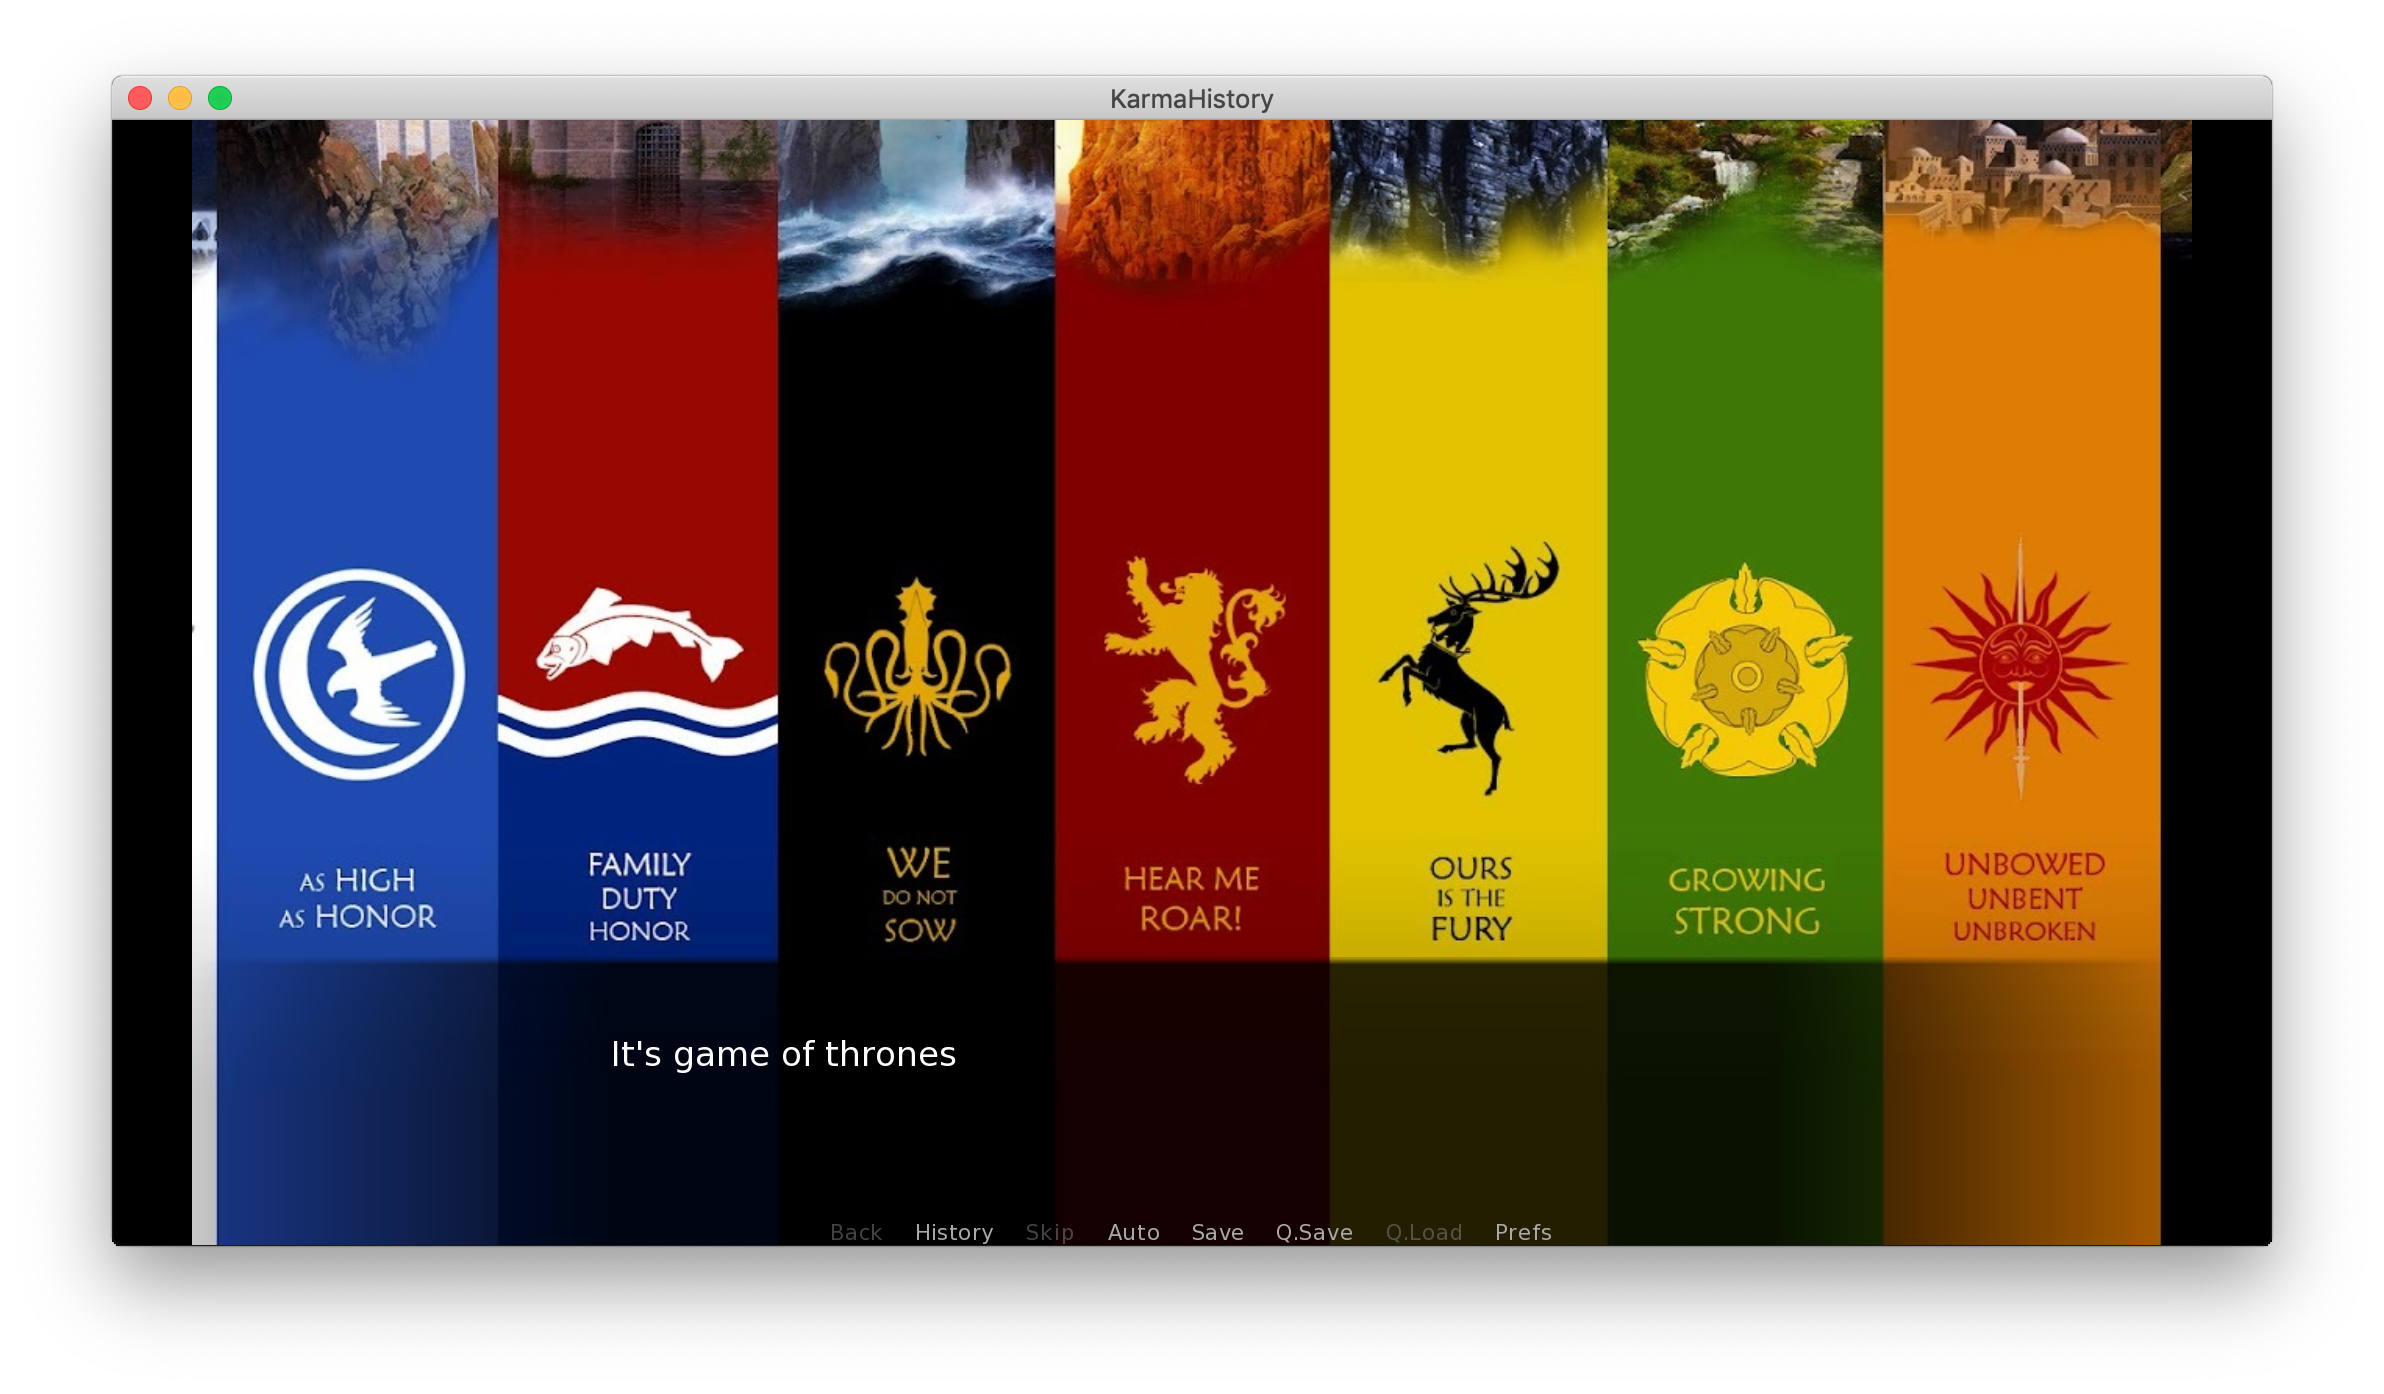
\includegraphics[width=0.4\textwidth]{images/gameStart.png}
    \caption{Opening screen for prototype game.}
    \label{fig:gameStart}
\end{figure}

\begin{figure}[ht]
    \centering
    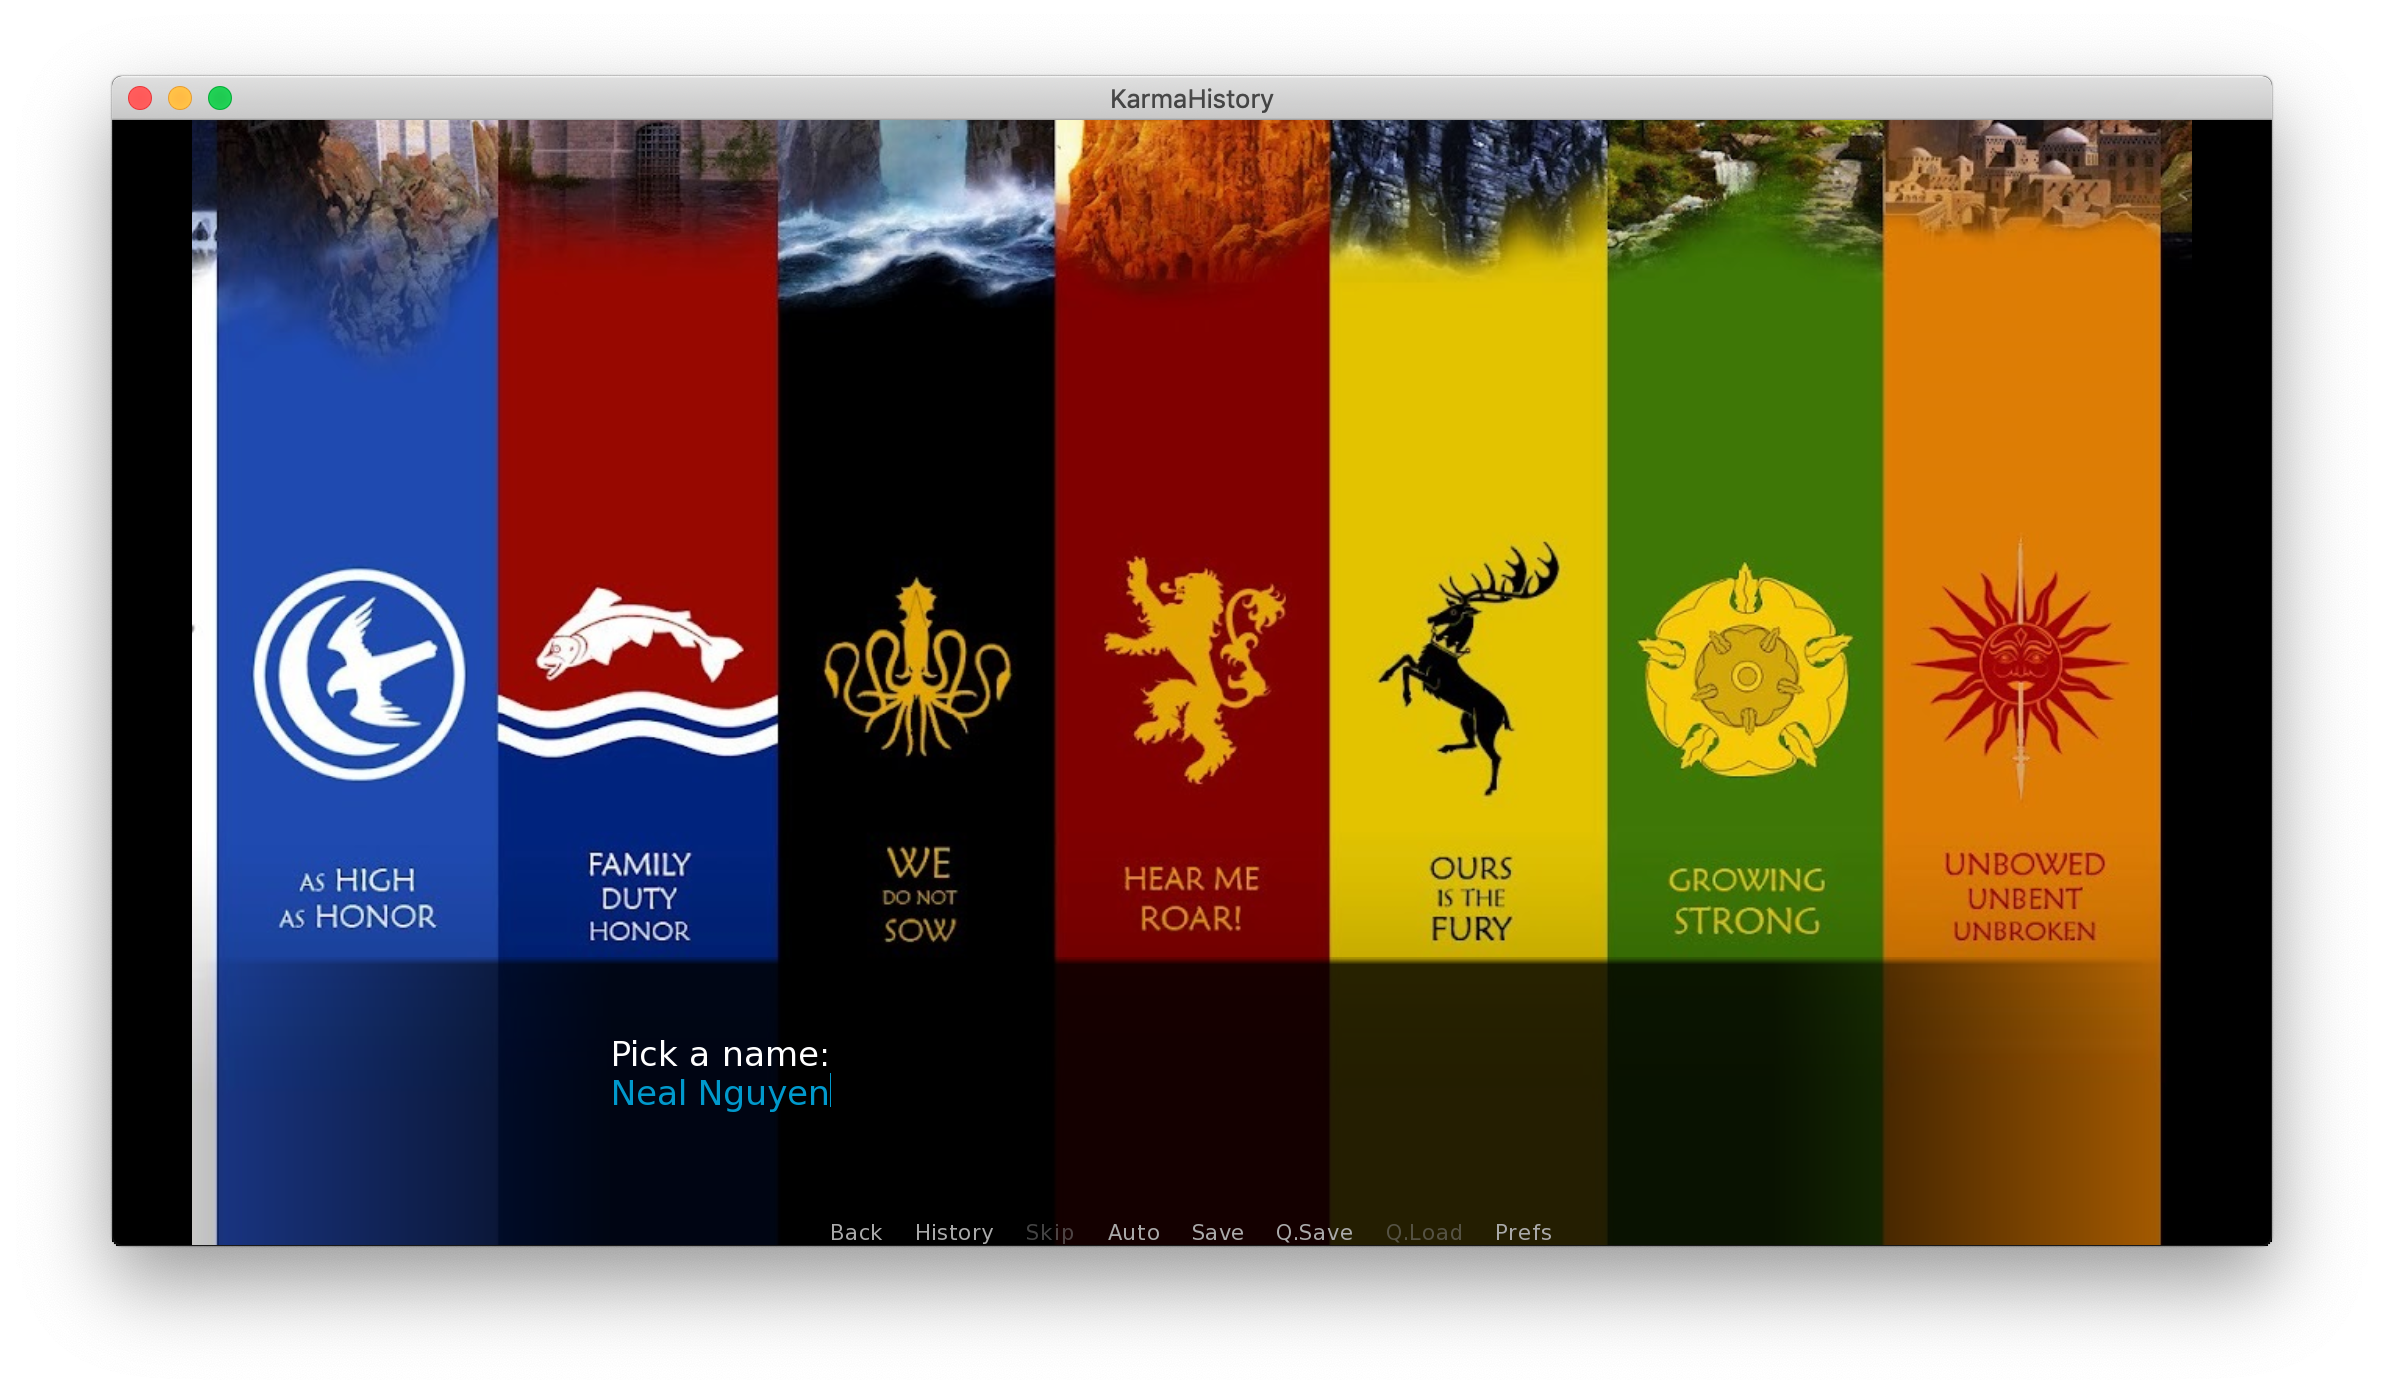
\includegraphics[width=0.4\textwidth]{images/chooseName.png}
    \caption{Entering player name for prototype game.}
    \label{fig:chooseName}
\end{figure}

\begin{figure}[ht]
    \centering
    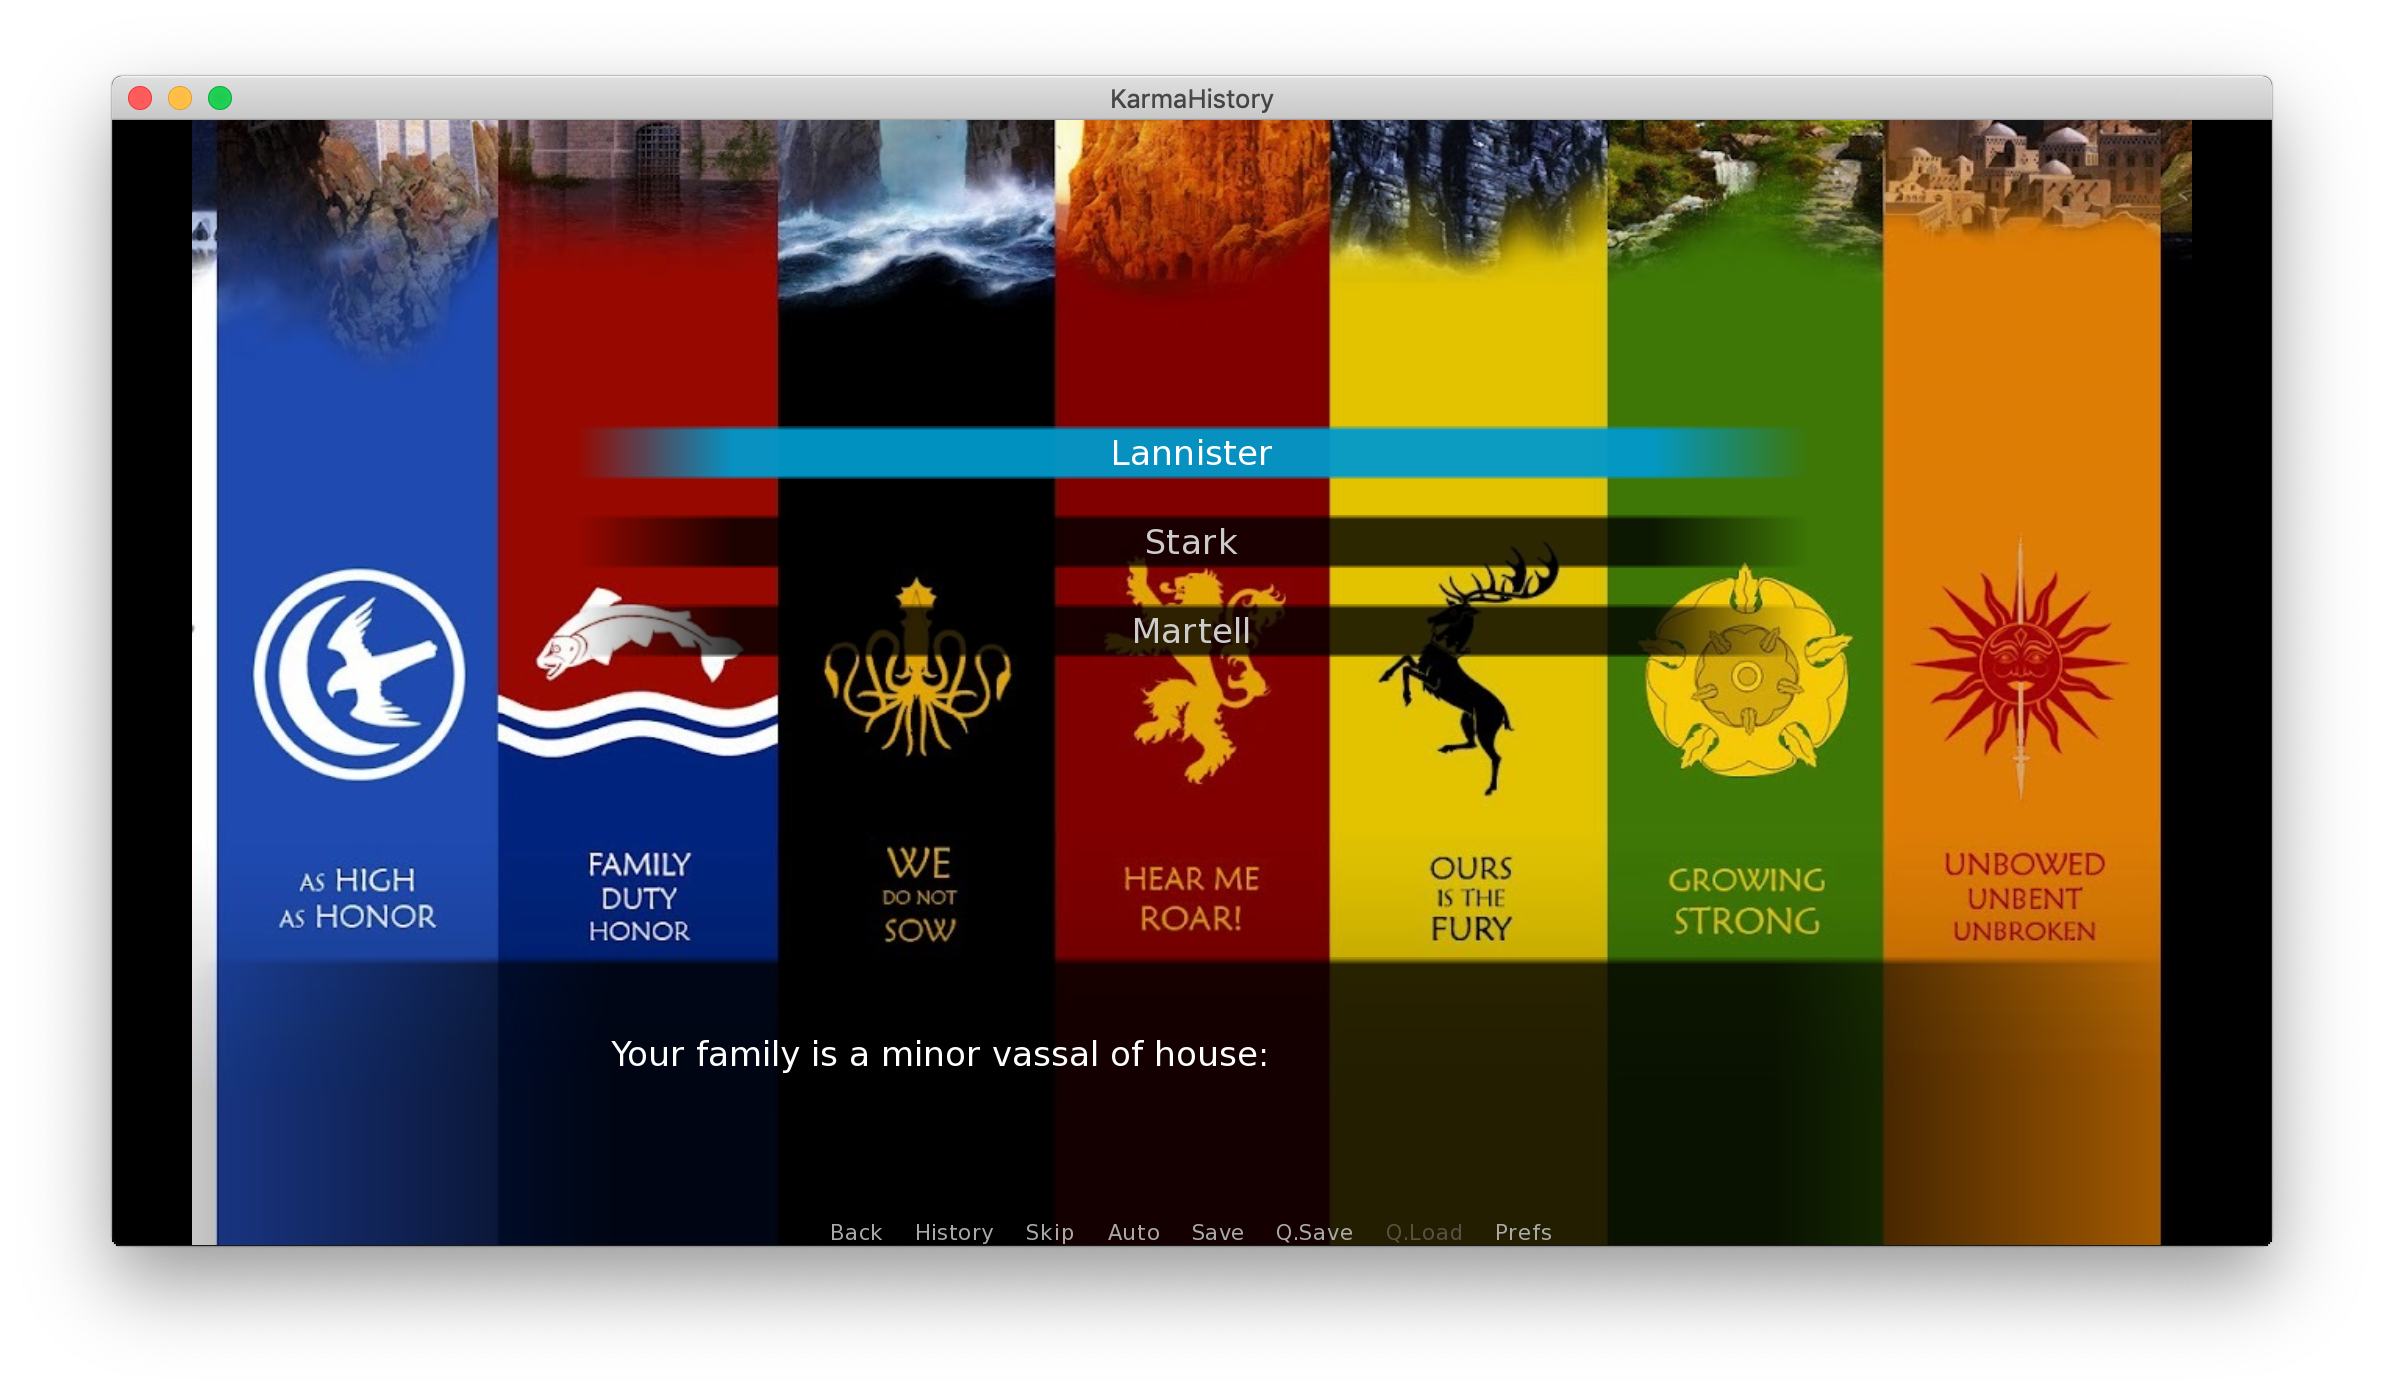
\includegraphics[width=0.4\textwidth]{images/chooseHouse.png}
    \caption{Choosing player house alliance for prototype game.}
    \label{fig:chooseHouse}
\end{figure}

\begin{figure}[ht]
    \centering
    \includegraphics[width=0.4\textwidth]{images/preGame.png}
    \caption{Static pregame at the beginning of each play through to calibrate player personality.}
    \label{fig:preGame}
\end{figure}

\begin{figure}[ht]
    \centering
    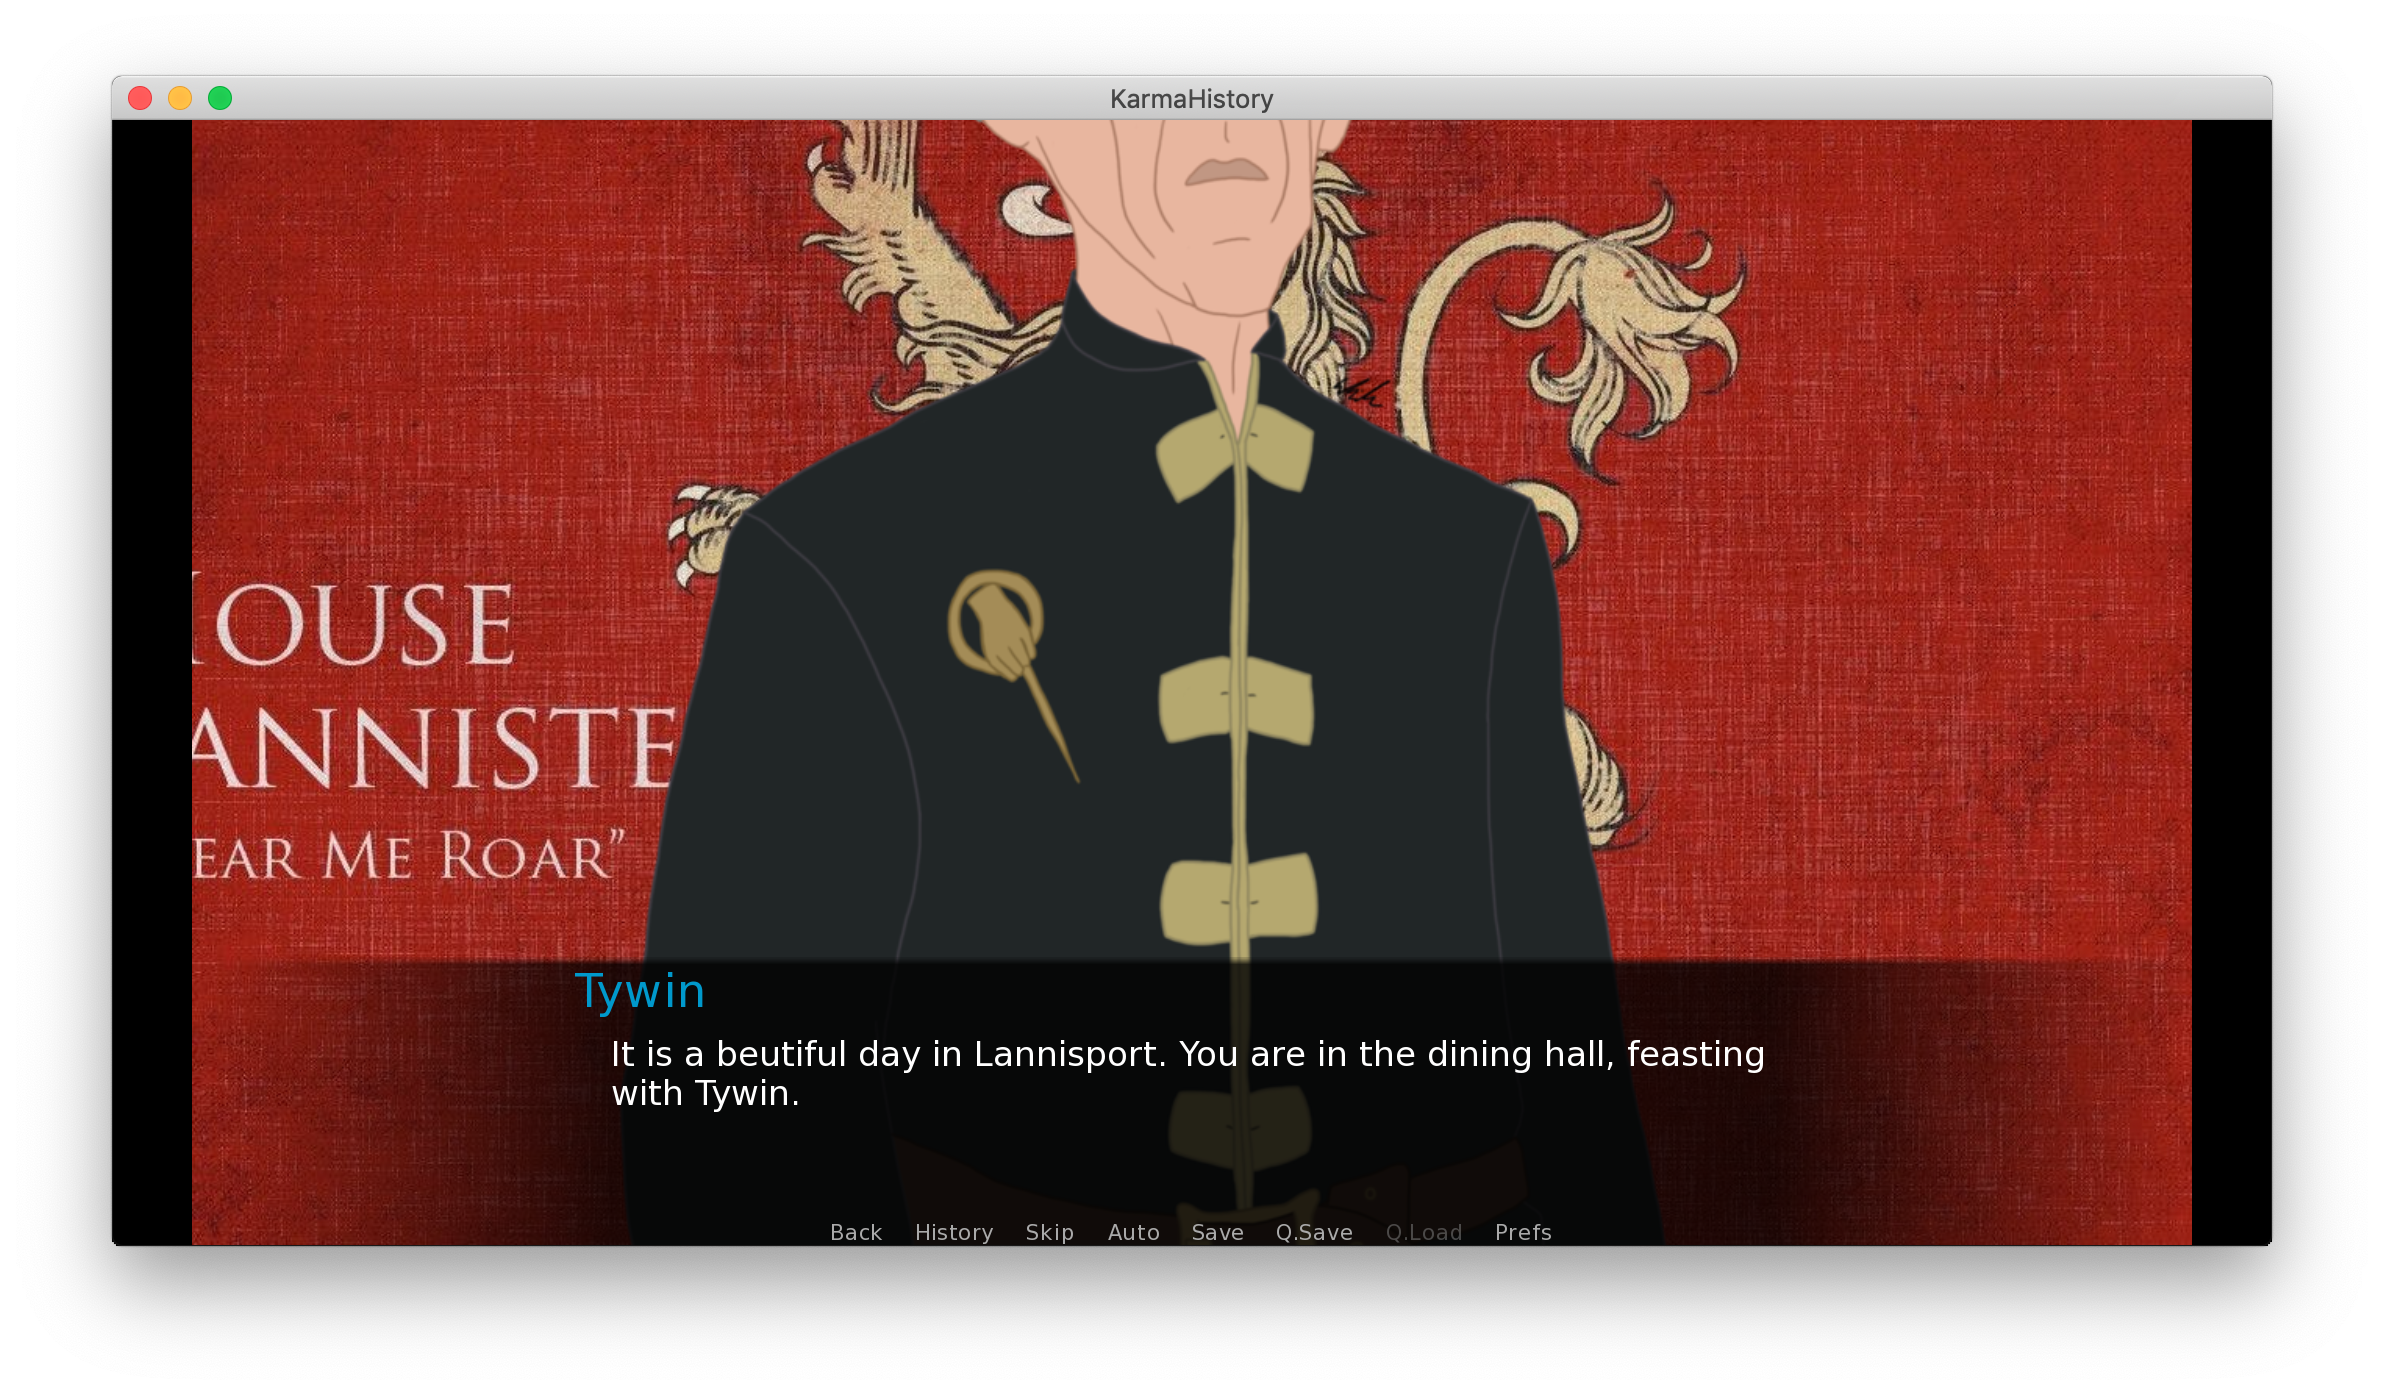
\includegraphics[width=0.4\textwidth]{images/customLannister.png}
    \caption{Start of adaptive PCG prototype pregame after house is chosen and personality is calibrated}
    \label{fig:customLannister}
\end{figure}